\section{Results}
\subsection{Application of RNAscape to structures from the PDB}

We present RNAscape output for various structures (Figures 1 and 4) from the PDB (21). In Figure 1A, tRNA from Sulfolobus tokodaii (PDB ID: 7VNV) is shown. RNAscape output preserves the L-shaped topology (as opposed to known ‘clover leaf’ shaped secondary structure (26) visualizations) and annotates non-standard bases and base-pairing geometries (critical in many RNA interactions (27)). RNAscape can also process unusual DNA structures, as shown by a single-stranded DNA with circular topology (PDB ID: 4NOE, Figure 1B). In Figure 1C, Dengue virus RNA promoter (PDB ID: 7UMD) is depicted, which is a single-stranded RNA molecule containing only standard RNA bases.

We present a few different examples of ribozymes and riboswitches (Figure 1D-G). RNA loop modeling (28) for riboswitches is an important area of research, and RNAscape visualizations (e.g. PDB IDs: 1Y26, 4FRN, 8HBA, Figure 1E-G) may aid in these efforts. The pistol ribozyme (PDB ID: 6R47, Figure 1D) and the Nicotinamide Adenine Dinucleotide-II (NAD-II) riboswitch (PDB ID: 8HBA, Figure 1G) illustrate how RNAscape places non-helical segments and can clearly depict their non-standard base pairs with helical segments. RNAscape natively supports multiple strands (e.g. PDB ID: 1Y26, Figure 1E). RNAscape is also able to visualize G-quadruplexes (PDB ID: 2M18, Figure 1E). An RNA structural motif which can serve as a binding site for proteins is the kink-turn motif (PDB ID: 7EFG) (29), and it is visualized in Figure 1I.

There has been a continued interest in structural studies of the ribosome which postulate the role of a proto-ribosome (30) in the origin of life. The proto-ribosome is a semi-symmetrical core of the ribosome comprised of RNA molecules representing the site for peptide bond formation, therefore known as peptidyl transferase center (PTC). The RNAscape visualization (Figure 1J, Supplementary Figure S1) for the same reflects the high degree of conformational symmetry, based on structural coordinates of the PTC provided by Bose et al. (30).

RNAscape can run on relatively large structures (structures of up to 50 MB are processed by the webserver). In Figure 4, we demonstrate its application to four different topologies of larger structures. In Figure 4A, a triangular topology of Mycobacterium tuberculosis ileS T-box in complex with tRNA (PDB ID: 6UFH, 244 nucleotides) is shown, followed by a diamond-like topology of mutant P4-P6 domain of Tetrahymena thermophila group I intron (PDB ID: 1HR2, Figure 4B, 157 nucleotides) and an exon free state of the Tetrahymena group I intron (PDB ID: 7R6N, Figure 4C, 354 nucleotides). Secondary structure representations will not resemble the structure at all for many of these cases (e.g. stacked ladders, PDB ID: 7QDU, Figure 4D, 552 nucleotides), while RNAscape is able to reflect the 3D topology of these large RNA molecules.
\begin{center}
    \begin{figure}
    \makebox[\textwidth]{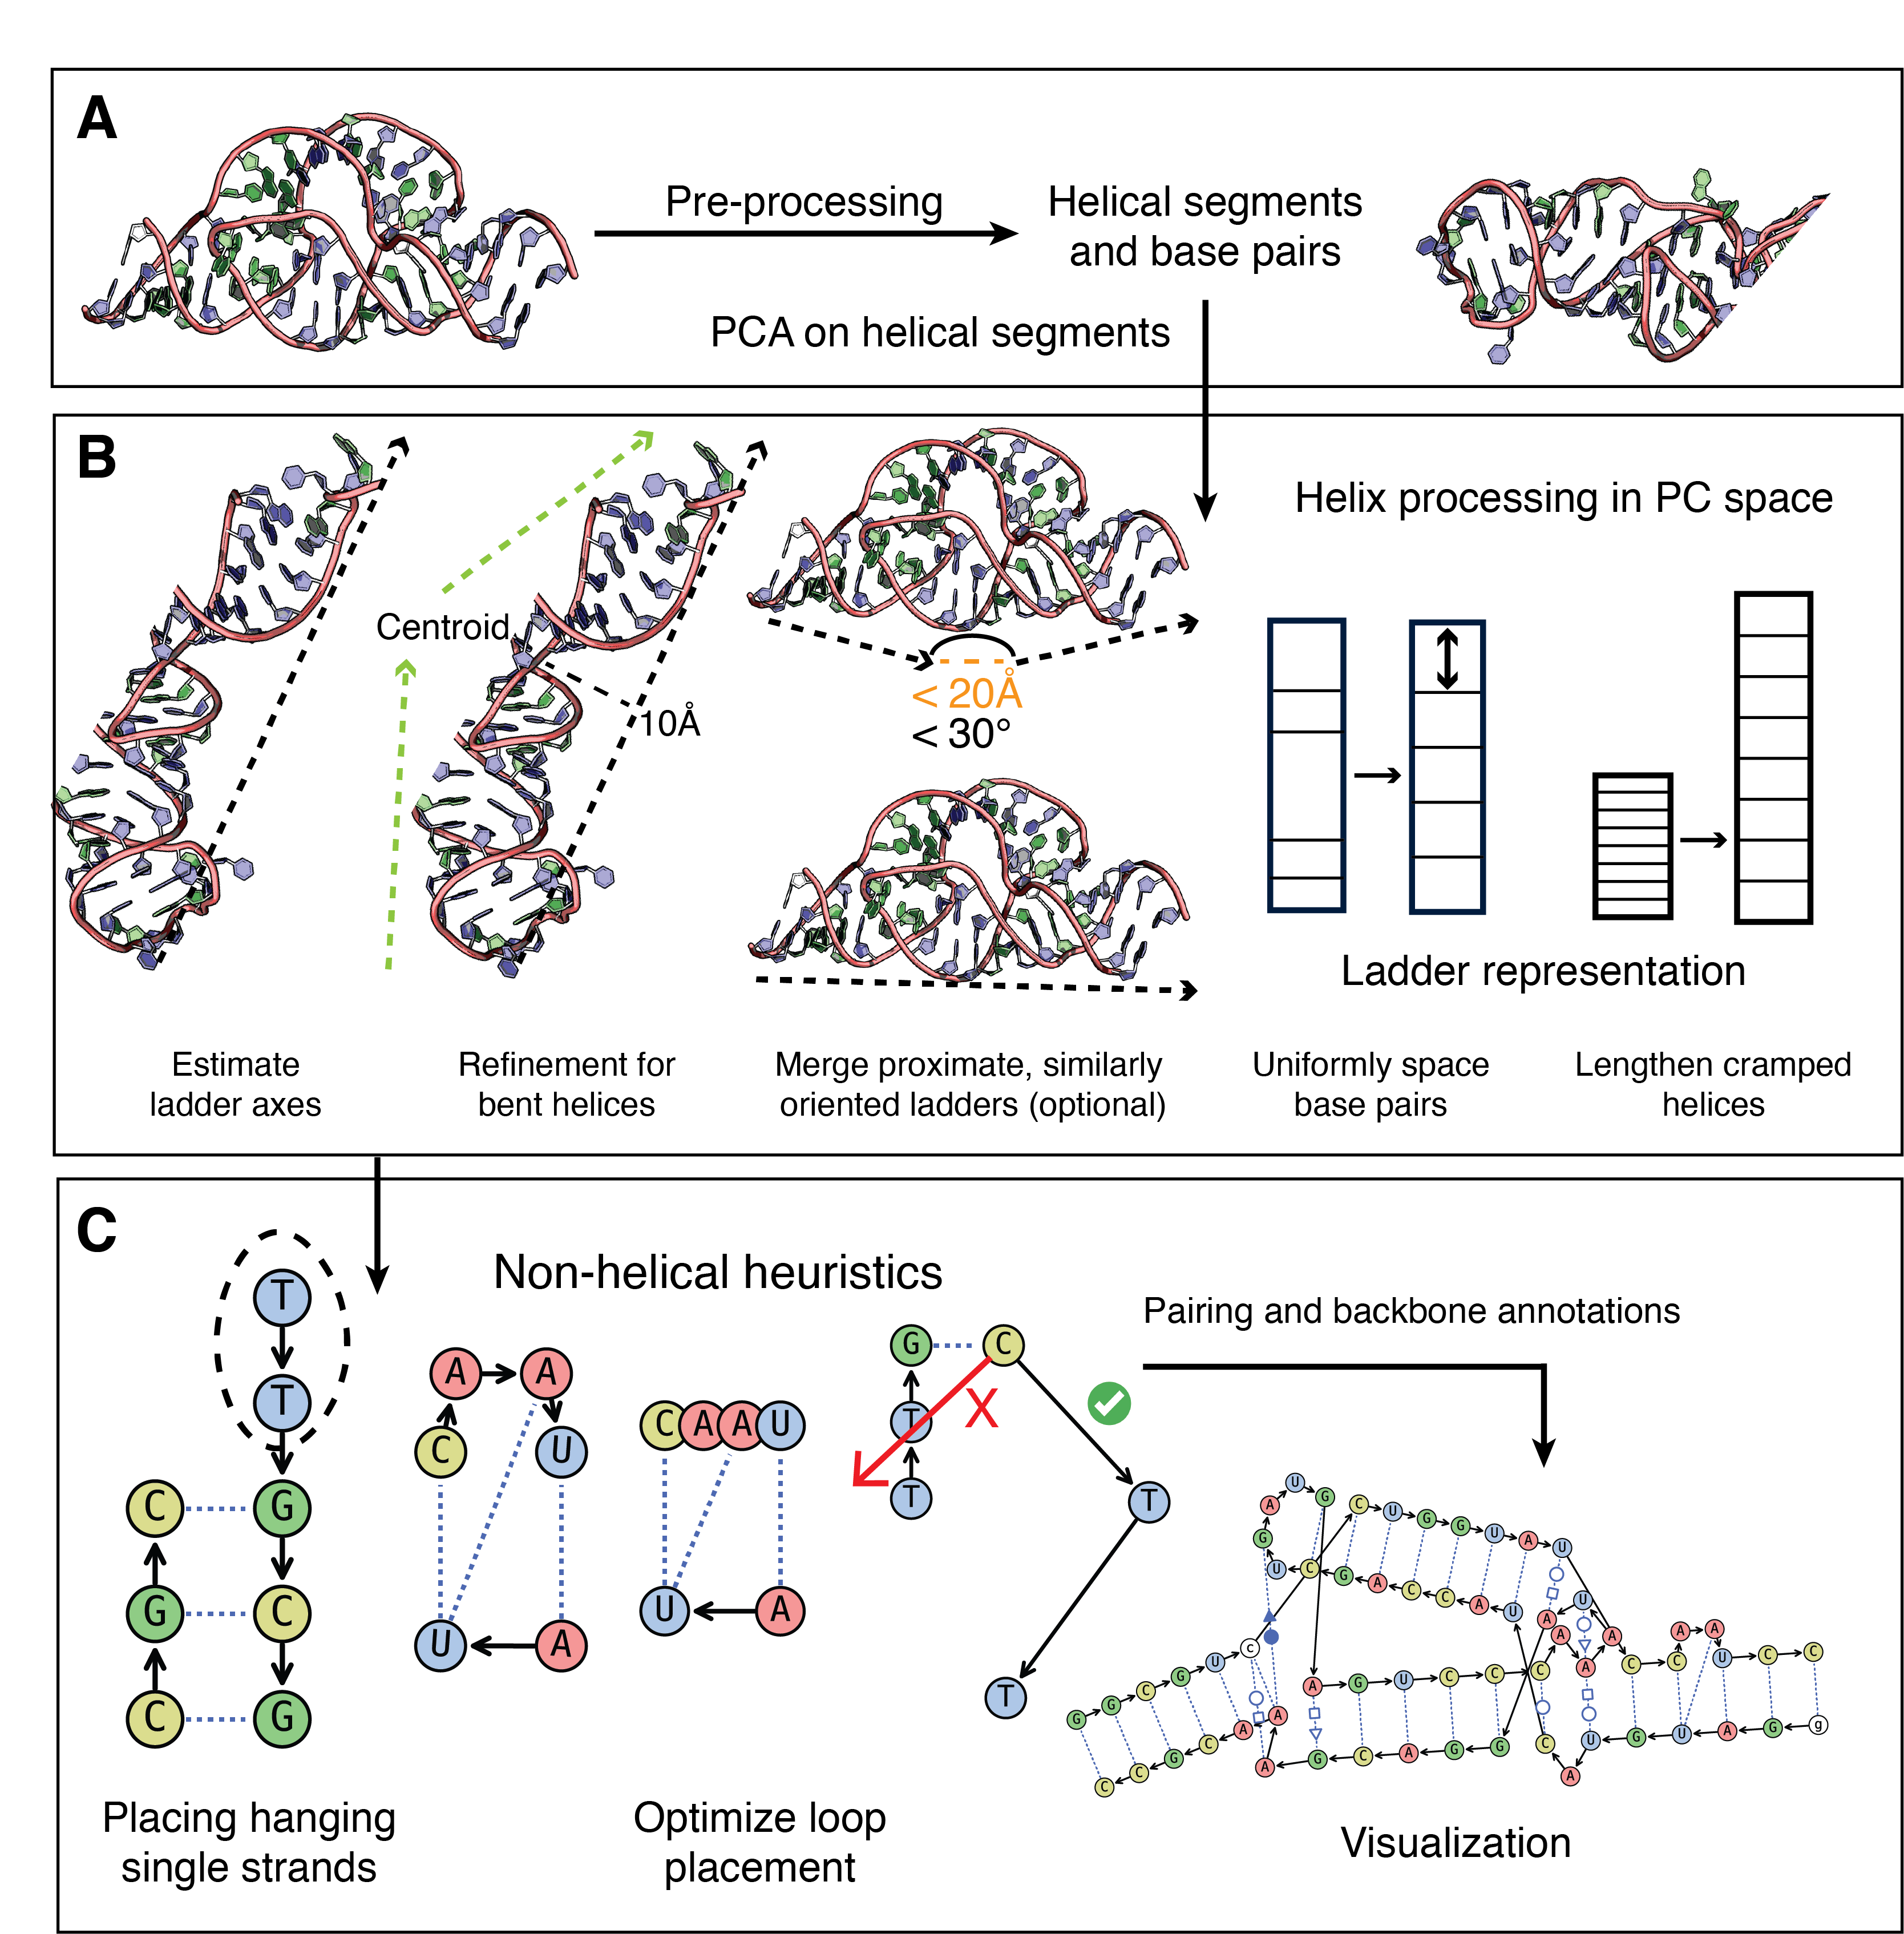
\includegraphics[width=0.8\paperwidth]{./rnascape\_figs/figure3.png}}
 % archetecture.png: 1149x508 px, 72dpi, 40.53x17.92 cm, bb=0 0 1149 508
        \caption[Computational cost of training RVAgene]{\textbf{Training RVAgene is reasonably scalable on CPU and even more so using hardware acceleration through GPU.} ({\bf A}) Time cost of training RVAgene for 100 epochs for datasets with varying number of genes and time points on CPU and GPU. ({\bf B}) Maximum memory utilized during training of the model on CPU an GPU for the cases in (A), inset plot: comparison of max memory used compared to DPGP for varying number of genes.}
  \label{fig:rnascape3}
\end{figure}
\end{center}
\subsection{RNAscape user interface}

The RNAscape webserver (Figure 2C) displays three primary items: header, file upload, and documentation panels. In the header, a user can click the ‘Run on Example Data’ button to view an example visualization (PDB ID: 3ZP8). In the file upload panel, a user can upload a structure using the file upload feature. This file may contain non-nucleic acid entities which will be ignored. Alternatively, a user can directly input a PDB ID to load its corresponding first assembly file. Clicking the ‘Run’ button runs the RNAscape pipeline on the uploaded structure file or provided PDB ID (biological assembly 1). After running RNAscape for a structure, a user has the option to add a second structure for side-by-side viewing. We demonstrate this capability for two structures of tRNA molecules (PDB IDs: 8UPT and 8UPY, Supplementary Figure S2), introduced by recent work (31) on the importance of tRNA shape. The documentation panel enables easy navigation and provides a quick start guide, tips, and examples for using RNAscape. It also includes detailed explanations for configurable settings.

\subsection{Output images}

The frontend (Figure 2C) natively supports touch-screen compatible image exploration. A user can zoom, center, or reset any zooming/panning via buttons above the display box. The image can also be rotated using a slider, and a ‘regenerate’ button is offered that replots the image, associated annotations, and user customizations in the desired rotation. To the right of the image, a legend is displayed that corresponds to the base-pairing annotation selected by the user. For the Saenger (19) base-pairing annotation, no legend is shown. The local strand direction ($5'$ to $3'$) is indicated by the black arrows between nucleotides for all plots. Other interactions are shown in blue dotted lines. These colors are fully customizable by the user. The user also has the option of downloading RNAscape mapped points in a numerical format (.npz) processable by the NumPy (32) library. Additionally, a log is provided which contains a description of the non-standard/modified nucleotides in the plot and other associated information.

\subsection{Base-pairing annotations}

RNAscape offers three base-pairing annotation styles: LW (16,33), DSSR (20) and Saenger (19). All base-pairing annotations are calculated via DSSR, although any future updates to these conventions by the nucleic acid community can be easily incorporated. Annotations do not affect geometric mapping, and a user can forego an annotation altogether. The LW annotation contains two key parameters: bond orientation (cis/trans) and base edge type. Bond orientation is represented by a filled or unfilled marker. The edge types: Watson-Crick (W), Hoogsteen (H), or sugar (S), are represented by marker shapes (Figure 1).

The DSSR style differs in that base edges are delineated by major groove (M), minor groove (m), or Watson-Crick (W) edges. Bond orientation annotation is the same as in the LW (16,33) annotation. DSSR also reports local strand orientation as a base-pairing annotation feature. RNAscape always denotes local strand orientation by the backbone arrows (Figure 1). Non-standard pairings flagged as ‘not categorized’ by DSSR are not annotated. For the Saenger (19) annotation, each bond type is represented by a number corresponding to its Roman numeral annotation.

\subsection{Customizable settings}

Several custom settings options are available (Figure 2C). The Loop Bulging setting controls whether loops are bulged outwards or linearly interpolated (see Materials and Methods). Additionally, the post-processing step of merging proximate, similarly oriented ladders can be turned off (Figure 3B). Since these settings affect the geometric mapping, a user must click ‘Run’ to run the pipeline again if they are changed. Arrow size, circle size, and circle label size affect nucleotide appearance. Base-pairing marker sizes can also be adjusted. Through the number settings, a user instructs RNAscape to label residue numbers in the numbering schema defined by the structure file. Color, size, frequency, and spacing of these labels can also be modified. Color settings allow a user to customize the color of each nucleotide type: A, C, G, U/T and X (non-standard nucleotides). Colors used to denote both backbone chain and non-chain interactions and markers can also be modified. Furthermore, RNAscape provides a functionality to modify calculated maps. By clicking on the ‘Modify Mapping’ button, the user can move and adjust nucleotide locations to resolve, for instance, overlap and regenerate the output.
\begin{center}
    \begin{figure}
    \makebox[\textwidth]{\includegraphics[width=0.7\paperwidth]{./rnascape\_figs/figure4.png}}
 % archetecture.png: 1149x508 px, 72dpi, 40.53x17.92 cm, bb=0 0 1149 508
        \caption[Computational cost of training RVAgene]{\textbf{Training RVAgene is reasonably scalable on CPU and even more so using hardware acceleration through GPU.} ({\bf A}) Time cost of training RVAgene for 100 epochs for datasets with varying number of genes and time points on CPU and GPU. ({\bf B}) Maximum memory utilized during training of the model on CPU an GPU for the cases in (A), inset plot: comparison of max memory used compared to DPGP for varying number of genes.}
  \label{fig:rnascape4}
\end{figure}
\end{center}

\section{Discussion}

The RNAscape webserver produces customizable, publication-quality visualizations of nucleic acid tertiary structure. It prioritizes the topology of a structure while striving to create a clean and optimized output, and it is designed to minimize user effort. RNAscape significantly deviates from any existing method in terms of its output quality, usability, and layout algorithm (Supplementary Table S1, Supplementary Figures S1 and S3). Users can refine visualizations on the webserver, and RNAscape also supports non-standard nucleotides and various base-pairing annotations. Further updates to base-pairing conventions may be easily incorporated. The RNAscape webserver allows a maximum file size of 50 MB. While potentially informative, the output for extremely large structures may not be well suited for presentation. We provide the RNAscape implementation via GitHub (see Data Availability) for those inclined to try the pipeline locally on even larger structures. We conclude with the hope that our effort facilitates advancement of the ever-growing field of RNA biology.